% Workshop version of paper/DRAFT.md (4 pages main text + references + appendix).
% Generic layout (NeurIPS-like text block); swap in the venue's style file once a venue is chosen.
% Build:  cd paper/workshop && tectonic main.tex
\documentclass[10pt]{article}
\usepackage[letterpaper,textwidth=5.5in,textheight=9in,top=1in]{geometry}
\usepackage[T1]{fontenc}
\usepackage{lmodern}
\usepackage{microtype}
\usepackage{amsmath,amssymb}
\usepackage{graphicx}
\usepackage{booktabs}
\usepackage{xcolor}
\usepackage[numbers,sort&compress]{natbib}
\usepackage[hidelinks]{hyperref}
\usepackage[font=small,labelfont=bf,skip=3pt]{caption}
\usepackage{enumitem}
\setlist{nosep,leftmargin=*}
\setlength{\textfloatsep}{8pt plus 2pt minus 2pt}
\graphicspath{{../figures/}}
\newcommand{\E}{\mathrm{E}}

\title{The Retrain Never Saw the Label:\\an Ill-Posed Reference in Class-Unlearning Audits\\of Conditional Diffusion Models}
\author{Anonymous authors}
\date{}

\begin{document}
\maketitle

\begin{abstract}
Class unlearning in conditional generative models is judged against an exact retrain, often by comparing the two \emph{under the forgotten label}. When the label enters through a learned embedding, the retrain's row for that label receives no gradient and stays at its random initialisation, as it would under standard DiT, ADM and EDM training code. This reference is therefore a network's response to an untrained, seed-specific input.

On a CIFAR-10 class-conditional DDPM with three exact retrains for each of four classes, the removed-label reference does not reliably recognise a held-out retrain: scores are undefined or range from $-2.1$ to $2.2$ where $1$ is expected, and sharing one row across retrains does not fix this (pre-registered). Querying the null (classifier-free-guidance) label, which every model trains, gives held-out retrains $0.94$--$1.13$ on the three classes with enough signal, while retrains that removed a different class score below $0.2$.

In a pre-registered study, a zero-step edit that only re-draws the forgotten label's row passes a removed-label closeness-and-behaviour audit on 30--60\% of draws, a rate similar to that of held-out retrains (3/9, post hoc). Yet re-fitting that one row restores the class to ${\geq}\,95.5\%$ of samples, against ${\leq}\,24.5\%$ for retrains (exploratory). For the published FID$_O$ metric, which compares samples with one retrain and reports $0$ for the retrain itself, two exact retrains differ by $2.1$--$4.3\times$ the sampling floor, inflated $1.3$--$3.0\times$ by the forgotten label; on two of three classes the unmodified model is no farther from some retrain than the retrains are from each other (pre-registered).
\end{abstract}

\section{Introduction}
Machine unlearning asks for a model that behaves as if some data had never been seen \citep{cao2015,bourtoule2021}. Since exact unlearning in deep networks means retraining without the data, approximate methods are judged by their closeness to a retrain. For class unlearning in diffusion models, when a retrain baseline is reported, the comparison is made \emph{under the forgotten label}: generation rates, FID or losses of the removed class \citep{fan2024salun,chen2025sfd,zheng2026tai}. FID$_O$, for instance, compares the unlearned model's samples with one retrain's ``for all the classes'', the forgotten one included \citep{zheng2026tai}. We study audits that compare losses or outputs under that label. Rate-only audits have a homogeneous reference (retrains generate almost none of the class); they can be passed by suppression without erasure, for a different, known reason \citep{pham2023,zhang2024attack}.

But a retrain never saw that label. Its embedding row receives no gradient, and under Adam(W) without weight decay it is exactly the initial random vector (to float32 round-off). The retrain's ``behaviour on the forgotten class'' is the network's readout of an untrained, seed-specific random input. Retrain-referenced evaluation is known to be fragile \citep{hayes2024,triantafillou2024,georgiev2025,lanyon2025,ebrahimpour2025,kim2026}. We identify a concrete, checkable cause of this fragility for class removal, and a reference without it.

\textbf{Contributions} (all failed predictions are in App.~\ref{app:prereg}):
\begin{enumerate}
\item \emph{Mechanism.} In all 12 exact retrains (4 classes $\times$ 3 seeds) the removed-label row is untrained, and on every class the removed-label reference fails to recognise some held-out retrain. A shared row does not repair it.
\item \emph{Alternative.} Null-label plain $\E$, registered before the confirmatory data, recognises every held-out retrain on the three classes with $\mathrm{SNR}\ge1.5$ (on ship a registered homogeneity conjunct failed) and does not score retrains of other classes as removals.
\item \emph{Consequence (pre-registered).} Zero-step re-draws pass the removed-label audit in 30--60\% of draws although the class is one row re-fit away. FID$_O$ against one retrain has a retrain-to-retrain spread of the size of published method gaps and, on two of three classes, does not separate the unmodified model from a retrain.
\end{enumerate}

\section{Mechanism and audit statistic}
Let $\theta_0\sim A(D)$ be the original and $O^{(s)}\sim A(D\setminus D_k;s)$ an exact retrain with seed $s$ on the data without class $k$. The label is looked up in an embedding table whose rows are initialised $\mathcal N(0,I)$.

\textbf{Proposition (untrained row).} If label $k$ never occurs in $D\setminus D_k$, the loss does not depend on $e_k$, so $\nabla_{e_k}L\equiv0$ at every step. Under Adam(W) the moment estimates of $e_k$ remain $0$, so its update $\eta\,\hat m/(\sqrt{\hat v}+\epsilon)$ is $0$. Decoupled weight decay $\lambda$ only shrinks the row, $e_k(T)=(1-\eta\lambda)^Te_k(0)$ (App.~\ref{app:rows}). In the audited EMA weights the row drifts by $5$--$8\cdot10^{-4}$ (float32 averaging).

\textbf{Consequence.} $\varepsilon_{O^{(s)}}(x_t,t,k)$ is the retrain's response to an untrained random conditioning vector. Nothing in training constrains how a network reads such an input, so the removed-label seed floor should be heterogeneous and poorly calibrated, and the null-label floor, whose row every model trains, should be neither. The training code of DiT (\texttt{nn.Embedding}, AdamW, decay $0$), ADM (likewise) and EDM (one-hot$\,\to\,$\texttt{Linear}, Adam) also gives an absent class exactly zero gradient.

\textbf{Closeness.} Let $\ell_m(q,t)$ be the $\varepsilon$-MSE of model $m$ on query image $q$ at timestep $t$ under label $y$ (the forget label or the null label), with noise shared across models, and let $d(a,b)$ be the RMS loss difference over queries and $t\in\{50,200,400,600,800\}$. Then $\E(u)=\frac{d(\theta_0,O)-d(u,O)}{d(\theta_0,O)-d_\text{floor}}$, where $d(\cdot,O)$ averages over the reference retrains and $d_\text{floor}$ is the mean retrain-pair distance. Doing nothing gives $\E=0$; a model as close to the references as they are to each other gives $\E=1$. $\E$ is \emph{undefined} (no measurable trace) if $\mathrm{SNR}=d(\theta_0,O)/d_\text{floor}<1.2$. CIs bootstrap over queries. A \emph{standardised} variant divides each timestep's losses by that timestep's floor.

\textbf{Calibration test.} Scored against the other two, a held-out retrain should give $\E\approx1$ under a well-posed reference.

\section{Experiments}
\textbf{Setup.} We use a class-conditional DDPM \citep{ho2020} on CIFAR-10 \citep{krizhevsky2009}: a 6.48M-parameter U-Net trained for 40k steps (mixed precision) with batch 128 and AdamW (lr $2\cdot10^{-4}$, weight decay $0$), EMA $0.9999$ and CFG dropout $0.1$ \citep{ho2022cfg}. The label lookup is \texttt{nn.Embedding(11,256)} with the null token at index 10. There are three exact retrains per removed class: automobile and cat, where we found the issue post hoc; ship, registered before data; and truck, drawn at random by a registered RNG. Queries are 256 training and 256 test images of the class, plus near and far classes, with identical images and noise for every model.

\begin{figure}[t]
\centering
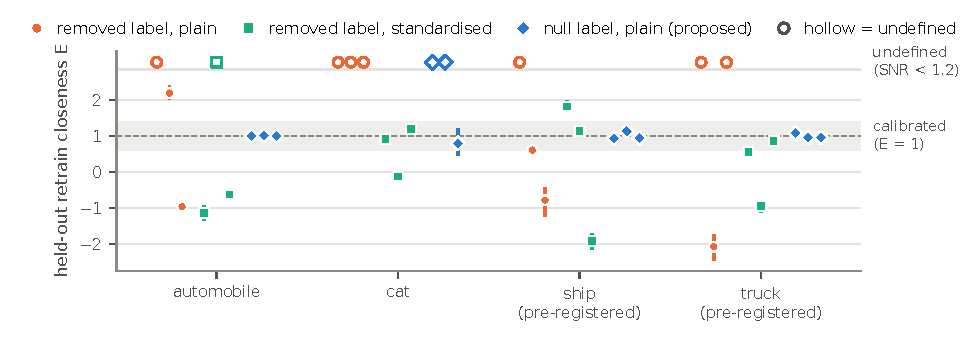
\includegraphics[width=\linewidth]{fig1_calibration.pdf}
\vspace{-1.5em}
\caption{\textbf{Calibration.} Each point is one held-out exact retrain scored against the other two; a well-posed reference gives $\E=1$. Shaded: $0.6$--$1.4$, the registered removed-label failure band; the registered null-label band is $[0.8,1.2]$. Bars: bootstrap 95\% CIs; hollow: undefined ($\mathrm{SNR}<1.2$). Cat lacks power under the null label ($\mathrm{SNR}\ 1.21<1.5$).}
\label{fig:calib}
\end{figure}

\textbf{The removed-label reference is ill-posed.}
\begin{itemize}
\item Every retrain's removed row stayed at its initialisation ($\le3.4\cdot10^{-6}$), while trained rows moved ${\approx}0.97$ (App.~\ref{app:rows}).
\item Under the removed label, the max/min retrain-pair distance at $t\le400$ is $16.1$ (automobile), $4.4$ (cat), $3.2$ (ship) and $6.6$ (truck).
\item Held-out retrains are undefined in 7 of 12 rotations under plain $\E$ and otherwise score $-2.08$ to $2.19$. Under standardised $\E$ they score $-1.92$ to $1.81$, with 4 of 12 inside $[0.6,1.4]$. Every class has at least one failing rotation (Fig.~\ref{fig:calib}); for ship and truck both failures were predicted before data.
\end{itemize}

\textbf{Sharing the row does not help (pre-registered C4-R; our predictions failed).} Transplanting retrains' removed rows ($3\times3$ grid per class), changing the row moves removed-label losses about as much as changing the network (ratio $0.69$--$1.71$ at $t\le400$), and a row shared by all three retrains neither halves the floor's max/min ratio on any class nor calibrates it (App.~\ref{app:prereg}).

\textbf{FID$_O$ against one retrain inherits this (pre-registered C4-F, C5).} FID$_O$ is the FID between the unlearned model's and one retrain's samples over all classes; \citet{zheng2026tai} report $0.00$ for the retrain. Computed as defined (2048-d, DDIM 50; 1{,}000 samples per label), two sampling runs of the original give $4.5$, while two exact retrains give $7.2$--$12.2$ (ship), $16.4$--$24.1$ (automobile) and $8.6$--$10.0$ (truck), and $5.8$--$8.8$ over the nine retained labels only. This spread matches published method values in size (SalUn $3.6$--$6.9$; scale only, as model, $n$ and guidance differ). On ship and automobile, $57\%$ and $93\%$ of re-draw--retrain values fall inside the retrain-pair range, and the unmodified original is closer to some retrain than the farthest pair ($8.6$ vs $12.2$; $11.6$ vs $24.1$), failing our registered sanity check. Truck's retrains agree more closely: the original separates ($11.6$ vs $10.0$) and $12\%$ of re-draws fall inside.

\textbf{The null-label reference is calibrated (plain $\E$, as registered).}
\begin{itemize}
\item Its pair ratio is $\le1.19$ at every $50\le t\le300$ on every class and $\le1.49$ in $t\le400$ (App.~\ref{app:timestep}). The window is post hoc: the registered rule, $\le1.3$ at every $t\le400$, failed on ship and truck.
\item Held-out retrains score $1.00$, $1.01$, $0.99$ (automobile); $0.94$, $1.13$, $0.94$ (ship); and $1.08$, $0.97$, $0.96$ (truck). All nine are inside the registered band $[0.8,1.2]$; 7 of 9 CIs contain $1$. Standardised null-label $\E$ (not registered) is not calibrated: $0.58$, $1.33$, $0.57$ on ship.
\item The trace is class-level (test-image SNR within 20\% of training-image SNR), specific (near and far classes have SNR $\le1.14$) and peaks at $t=100$--$200$ (registered).
\item It tracks removal of the class, not network identity (pre-registered C4-X): retrains that removed a \emph{different} class score $-0.41$ to $0.19$ (registered: all 27 $<0.5$).
\item Null-label SNR is $3.7$ (automobile), $2.4$ (truck), $1.9$ (ship) and $1.21$ (cat, below the registered power threshold $1.5$; Fig.~\ref{fig:calib}).
\end{itemize}

\begin{figure}[t]
\centering
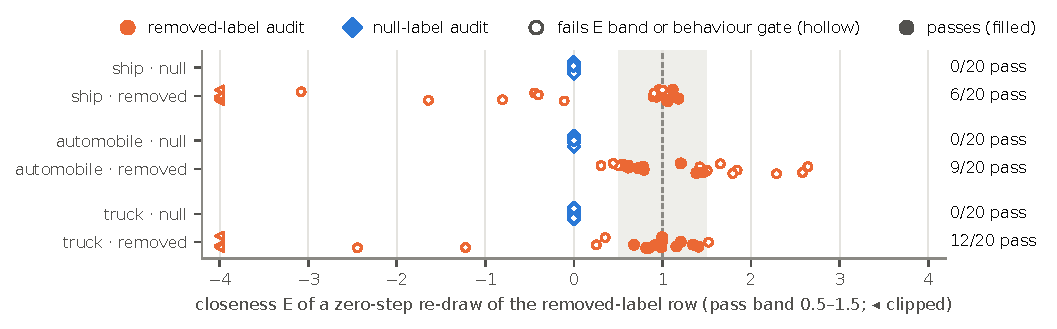
\includegraphics[width=\linewidth]{fig3_redraws_pass.pdf}
\vspace{-1.5em}
\caption{\textbf{A zero-step edit passes the removed-label audit (pre-registered).} We made 20 random re-draws of the forgotten label's embedding row per class, keeping all other weights. A model passes (filled) if $\E\in[0.5,1.5]$ \emph{and} its forget-class generation rate is at most the worst retrain's rate $+0.05$. Removed-label $\E$ is standardised, except plain for automobile (standardised SNR $1.18<1.2$; registered amendment).}
\label{fig:redraw}
\end{figure}

\textbf{Consequence: the audit can be passed without unlearning (pre-registered).} For ship, automobile and truck we audited doing nothing, 20 zero-step re-draws ($e_k\leftarrow\mathcal N(0,I)$), and five approximate methods with two seeds each (App.~\ref{app:methods}).
A re-draw replaces the trained row with a fresh random one, keeps every other weight, and removes nothing. Yet it passes the removed-label audit, on closeness \emph{and} behaviour, in $6/20$ (ship), $9/20$ (automobile) and $12/20$ (truck) draws (Wilson 95\% CIs $[0.15,0.52]$, $[0.26,0.66]$, $[0.39,0.78]$; Fig.~\ref{fig:redraw}).

Under the same rule, with leave-one-out references (two rather than three), 3 of 9 \emph{genuine} held-out retrains pass (0/3, 1/3, 2/3; post hoc). Re-draws and retrains pass at similar rates (27/60, 3/9), so the audit cannot tell them apart, as \S2 predicts: like a retrain, a re-draw reads the label through an untrained random vector.

Passing depends on the draw, so an auditee could pick a passing one. No re-draw or method is retrain-equivalent under the null-label audit (App.~\ref{app:methods}). All 12 registered predictions held (A2--A4 were low-risk; A1 is the test).

\begin{figure}[t]
\centering
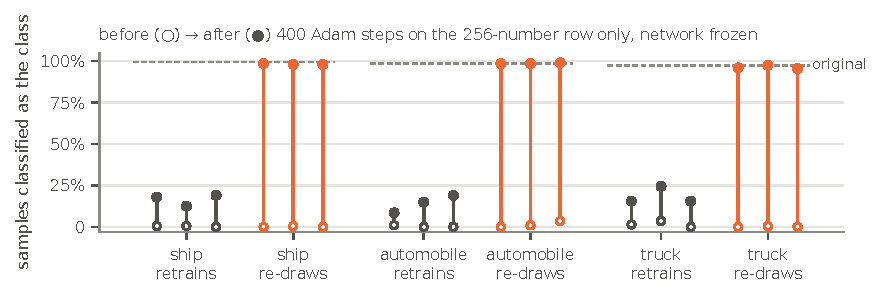
\includegraphics[width=\linewidth]{fig4_row_refit.pdf}
\vspace{-1.5em}
\caption{\textbf{The class is one row away (exploratory).} Only the removed label's row is fitted (network frozen; 400 Adam steps on 1{,}000 class images disjoint from the audit set), in re-draws that \emph{passed} the removed-label audit and in exact retrains. Dashed: the original's rate.}
\label{fig:refit}
\end{figure}

\textbf{The re-drawn models still contain the class (exploratory; predictions logged before running).} As the null-label score of $0$ holds by construction, we test recoverability. For three passing re-draws per class (App.~\ref{app:prereg}), re-fitting only the removed row restores generation of the class to $0.955$--$0.990$ in all 9, against the original's $0.975$--$0.995$. The same re-fit brings exact retrains only to $0.085$--$0.245$ (Fig.~\ref{fig:refit}). Unconditionally, the original generates the class at $4.3$--$14.5\times$ the retrains' rate (retrains: 2--19 of 1{,}000 samples). The null-label verdict is right.

\section{Recommendations and limitations}

\textbf{Recommendations.} (1) Do not use the retrain's removed-label pathway as a reference. If one is reported, add the seed spread, a leave-one-retrain-out check and zero-step re-draws as a negative control. For FID$_O$, report the retrain-to-retrain value, not $0$. (2) Where the model has a trained null token (DiT by default; EDM only with label dropout; not ADM), audit the unconditional pathway against several retrains; a held-out retrain should score ${\approx}1$. (3) State the conditioning and optimiser: learned input-side label embeddings are affected; frozen text encoders and output heads are not.

\textbf{Limitations} (App.~\ref{app:limits}; related work App.~\ref{app:related}): one U-Net; three retrains per class.
\bibliographystyle{abbrvnat}
\bibliography{refs}

\appendix
\section{Pre-registration record}\label{app:prereg}
Registrations with timestamps, unit-tested scoring code, the per-run log and a one-command figure script will be released with the paper.
\paragraph{How the mechanism was found (C1, negative).}
An earlier finding of ours on cat, replicated with three retrains, said the exact-retrain trace of class removal lives only at high noise. A pre-registered test on a fresh class (automobile) failed: there was no high-noise trace, and even on cat the standardised statistic did not recognise a held-out retrain ($\E=-0.18$ in the C1 pipeline; the later label-diagnostic recomputation plotted in Fig.~\ref{fig:calib} gives $-0.12$). Diagnosing this failure led to \S2. The cat pattern came from trained-versus-random conditioning on that class, not from class removal.

\paragraph{C2 (ship).} Registered before data. Held:
\begin{itemize}
\item a trace is present (SNR $1.85$);
\item calibration;
\item the trace is class-level and specific;
\item low/mid-noise localisation;
\item the removed-label reference fails in both predicted ways.
\end{itemize}
\textbf{Failed:} null-label homogeneity $\le1.3$ at every $t\le400$ (observed $1.42$ at $t=400$). Under the registered conjunctive rule, the calibration claim was therefore ``not confirmed as registered''.

\paragraph{C3 (registered before any C3 data).}
\begin{itemize}
\item \emph{C3-B} drew truck with a fixed RNG. It replaced the homogeneity rule with ``$\le1.5$ and below the removed-label ratio at every $t\le400$''; this held, with $1.49$ at $t=10$. The original $\le1.3$ rule failed again. With that rule replaced, the calibration claim is confirmed on truck.
\item \emph{C3-A}: all 12 predictions held (Fig.~\ref{fig:redraw}, Table~\ref{tab:c3a}). In closeness 10, 10 and 12 re-draws land in the band; in behaviour 10, 17 and 18 pass the gate. Median $\E$ is $0.40$, $1.30$, $0.88$; passing correlates across classes for the same vector (ship--truck $\rho=0.52$; 3 vectors pass on all three).
\item \emph{Re-fit (exploratory).} Adam, lr $0.05$, 400 steps, batch 64. We used the first three passing re-draws for automobile and truck; for ship, run first, we used the three passers with $\E$ closest to $1$ (102, 109, 110; not the first three, which include 108). Both choices were fixed before running.
\end{itemize}

\paragraph{C4 (registered before any C4 data).}
\begin{itemize}
\item \emph{C4-R (row swap), all three predictions failed; R1 held on cat and ship.} R1: the row out-moves the network at $\ge4$ of the 6 timesteps $t\le400$ on $\ge3$ of 4 classes (observed 2/6, 6/6, 4/6, 3/6). R2: a common row halves the max/min ratio on $\ge3$ classes (0 of 4). R3: common-row leave-one-out $\E\in[0.6,1.4]$ in $\ge2/3$ of defined rotations (no class). We therefore withdrew our earlier explanation, that the independent draws add a second source of variation.
\item \emph{C4-X (cross-class), held.} 27 of 27 null-label scores $<0.5$ (max $0.19$).
\item \emph{C4-F (Fréchet distance, ship, automobile, truck).} F1, held: $\ge25\%$ of re-draw--retrain FDs $\le$ the largest retrain-pair FD (0.73, 0.85, 0.28). F2, held: retrain pairs differ $>1.5\times$ more under label $k$ than under airplane (8.3, 16.3, 5.5). F3, the sanity check that the original is farther from every retrain than any retrain pair, failed on all three.
\end{itemize}

\paragraph{C5 (FID$_O$, registered before any C5 data).} O1, held (2/3): $\ge25\%$ of re-draw--retrain values $\le$ the largest retrain pair (0.57, 0.93; truck 0.12 failed). O2, held (3/3): mean retrain pair $>1.5\times$ the sampling floor (2.3, 4.3, 2.1). O3, the sanity check as in F3, \textbf{failed} (needed 3/3; held on truck only). O4, held (3/3): all-label retrain pairs $>1.25\times$ retained-only (1.49, 3.02, 1.28).

\begin{table}[h]
\centering\footnotesize\setlength{\tabcolsep}{4pt}
\caption{C3-A (pre-registered). Prediction IDs in parentheses.}
\label{tab:c3a}
\begin{tabular}{lccc}
\toprule
& ship & automobile & truck\\
\midrule
re-draws passing (A1, $\ge1$) & 6/20 & 9/20 & 12/20\\
SD of re-draws' $\E$ (A2, $\ge0.3$) & 4.77 & 0.72 & 3.03\\
highest null-label lower CI over method $\times$ seed (A3, $<0.8$) & $-0.85$ & $-0.29$ & $0.16$\\
label annealing, null-label $\E$ (A4, $<0$) & $-1.87$, $-1.87$ & $-0.79$, $-0.81$ & $-1.33$, $-1.34$\\
\bottomrule
\end{tabular}
\end{table}

\section{Related work}\label{app:related}
Some diffusion-unlearning work reports forget-label generation without a retrain baseline \citep{heng2023,wu2024erasediff}. Where a baseline is used, we found no discussion of what the retrain's forgotten-label pathway is. On the fragility of retrain-referenced evaluation:
\begin{itemize}
\item population-level membership attacks overestimate protection \citep{hayes2024};
\item results vary with training randomness \citep{triantafillou2024,georgiev2025,lanyon2025}, as does FID itself \citep{dufour2026fid};
\item retrain-vs-retrain comparison as a floor: on Stable Diffusion it is small \citep{cho2025fade}, as our mechanism predicts for a frozen text encoder, where the forgotten prompt is never an untrained input;
\item class-unlearning targets approximate the retrain's outputs \citep{ebrahimpour2025};
\item evaluation protocols have been re-examined more broadly \citep{kim2026}.
\end{itemize}
Erased text-to-image concepts can be recovered by textual inversion or adversarial prompts \citep{pham2023,zhang2024attack}; our row re-fit is a white-box analogue. Tokens absent from LLM training likewise receive no input-embedding gradient \citep{land2024}. In classifiers, by contrast, an absent class's \emph{output} row does receive gradient through the softmax \citep{zheng2026head}, so our mechanism is specific to input-side conditioning.

\section{Limitations (full)}\label{app:limits}
\begin{itemize}
\item \emph{Scale.} One 6.5M-parameter U-Net on CIFAR-10, with three retrains per class.
\item \emph{Statistics.} CIs are conditional on the reference retrains, and each leave-one-out floor comes from one pair; two of nine null-label CIs exclude $1$. Pass rates come from 20 draws per class, and the same vectors are reused across classes, so the classes are not independent replicates.
\item \emph{Power.} The null-label audit lacks power when other classes cover the removed one (cat).
\item \emph{Homogeneity.} Our registered homogeneity rule ($\le1.3$) failed on ship and truck, and its revision held on truck by $0.01$.
\item \emph{Methods.} The methods ran at one setting, where they collapse or barely forget, so we rank none of them.
\item \emph{Null-label audit.} It is shown to be specific, not sensitive. It has no positive control beyond retrains (retain-only fine-tuning already scores below $0$), it certifies only the unconditional pathway, and an edit confined to that pathway could in principle game it.
\item \emph{Mechanism attribution.} The row swap (C4-R) shows that the draw's identity is not the main driver. That the input being \emph{untrained} is the cause rests on the contrast with the trained null label; training the removed row in each retrain and re-measuring the floor would test it directly.
\item \emph{Generality.} DiT, ADM and EDM were checked at the code level only; we did not train them. The null-label alternative needs a trained null token: DiT trains one by default, EDM only with \texttt{label\_dropout}$\,>0$ (default $0$), and ADM has none.
\item \emph{Retained labels.} We audit the null pathway only. Knowledge of class $k$ could survive in a retained label's pathway; auditing every trained label would be more complete.
\item \emph{Small counts.} The unconditional-rate ratio rests on 2--19 class samples per retrain out of 1{,}000.
\item \emph{FID$_O$.} We used 1{,}000 samples per label (Zheng et al.\ use 5{,}000) and one guidance scale; FID is biased upward at small $n$, so our values are not numerically comparable with published ones. Retained-label-only retrain pairs also exceed the sampling floor, so part of the spread is general training-seed variance, not the forgotten label. The pattern is class-dependent (truck separates the original).
\item \emph{Scope.} Text-to-image models with frozen text encoders are outside the mechanism.
\end{itemize}

\section{The removed-label row never moves}\label{app:rows}
\begin{center}
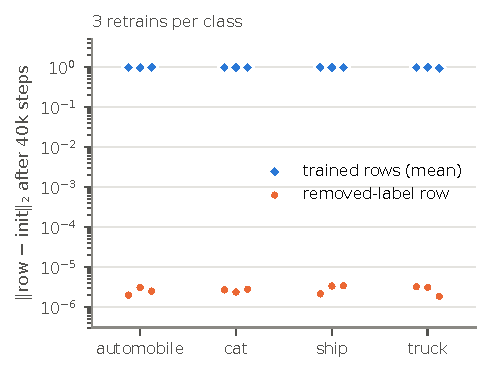
\includegraphics[width=0.55\linewidth]{fig2_untrained_row.pdf}
\end{center}
Distance from initialisation after 40k steps, for every exact retrain. Re-initialising each retrain from its seed reproduces the row to float32 round-off. Trained rows move only ${\approx}6\%$ of their norm. Gradient clipping does not affect the untrained row. Large $\eta\lambda T$, or coupled L2, would instead drive the row towards $0$ in every retrain, which changes the failure mode. In the EMA weights it drifts by $5$--$8\cdot10^{-4}$ (${\approx}4\cdot10^{-5}$ relative) through float32 averaging.

\section{Per-timestep heterogeneity}\label{app:timestep}
\begin{center}
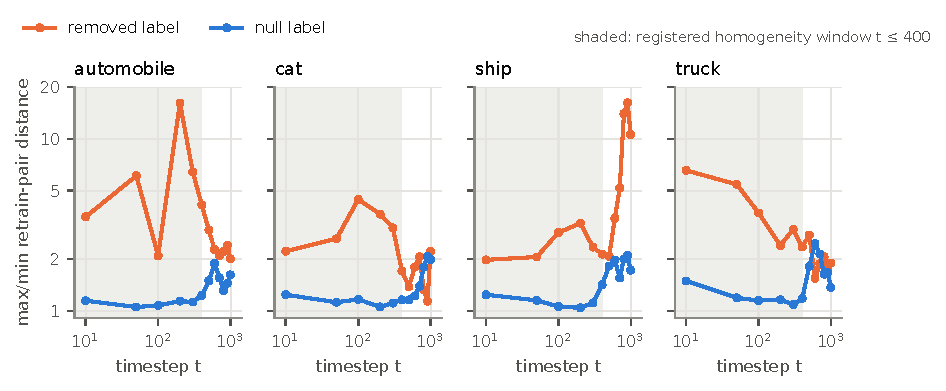
\includegraphics[width=\linewidth]{fig5_pair_heterogeneity.pdf}
\end{center}
Max/min of the three retrain-pair distances per timestep, on training images of the removed class. The shaded region is the registered homogeneity window $t\le400$. Within it, the removed-label floor is heterogeneous on every class, while the null-label floor is near $1$ at $50\le t\le300$ (truck reaches $1.49$ at $t=10$). The audit statistic also uses $t=600$ and $800$, where the null floor is heterogeneous too (up to $2.5$; on truck at $t=600$ it exceeds the removed-label ratio). Plain $\E$ is dominated by the larger loss differences at low $t$.

\section{Unlearning methods (exploratory, not registered)}\label{app:methods}
\begin{itemize}
\item \emph{Hyper-parameters.} 2000 steps at lr $3\cdot10^{-5}$.
\item \emph{Gradient ascent and variational EWC} reach a zero forget rate by collapsing the model ($|\E|$ in the hundreds or more on both audits).
\item \emph{Gradient difference} collapses on the removed label. On ship and truck it is the closest method on the null label, though on truck that cell's class samples are 100\% degenerate; on automobile, retain fine-tuning is closer.
\item \emph{Label annealing} (our diffusion adaptation of a classifier method, \citealp{panda2025}) \emph{and retain fine-tuning} barely forget (forget rate $0.89$--$1.00$). Under the null-label audit, label annealing, which trains the null label on forget images, moves \emph{away} from the retrain ($\E$ $-0.8$ to $-1.9$, registered prediction A4), further than retain fine-tuning ($-0.24$ to $-0.74$); the null-label $\E$ thus also penalises generic drift.
\item \emph{Degenerate outputs.} Classifier-based forget rates must be gated: in one cell (gradient difference, cat, seed 0), 65\% of saturated-noise samples were labelled ``cat'' by the CIFAR-10 classifier.
\end{itemize}

\end{document}
